\documentclass{mcmthesis}
\usepackage{ctex}
\mcmsetup{tstyle=\color{red}\bfseries,%修改题号，队号的颜色和加粗显示，黑色可以修改为 black
        tcn = 2600043, problem = F, %修改队号，参赛题号
        sheet = true, titleinsheet = false, keywordsinsheet = true,%修改sheet显示信息
        titlepage = false, abstract = true}



  %四款字体可以选择
  \usepackage{times}
  %\usepackage{newtxtext,newtxmath} %CTeX 无此字体，可用 txfonts 替代，请使用新版 TeXLive.
  %\usepackage{palatino}
  %\usepackage{txfonts}

%\usepackage{indentfirst}  %首行缩进，注释掉，首行就不再缩进。
\usepackage{lipsum}
\usepackage{etoolbox}
\usepackage{booktabs}
\usepackage{tabularx}   % optional (not used below)
\usepackage{arydshln}   % for dashed rules: \cdashline
\usepackage{caption}
\usepackage{float} 
\usepackage{booktabs} % 用于表格美观横线，必加
\title{用还是不用生成式AI？这就是问题！}



\date{\today}
\renewcommand{\contentsname}{\rmfamily 目录}
\pretocmd{\tableofcontents}{\begingroup\rmfamily}{}{}
\apptocmd{\tableofcontents}{\endgroup}{}{}

\begin{document}


\begin{abstract}
\par 请使用该模板开始撰写电子报告的第一页（Summary Sheet）。本模板默认使用 12 号 Times New Roman 字体。请以 Adobe PDF 电子文件形式提交论文（例如 1111111.pdf），使用英文撰写，并确保字体清晰可读且字号不小于 12 号。

请不要在本页或任何页面包含学校名称、指导老师或队员姓名等可识别信息。

请务必在上方修改控制号（control number）与题号（problem choice）。

当开始正式写作时，可删除这些说明文字。

\textbf{请关注我们的社交媒体 @COMAPMath（Twitter）或 COMAPCHINAOFFICIAL（微博），以获取最新竞赛信息。}

\begin{keywords}
关键词1; 关键词2
\end{keywords}
\end{abstract}



\maketitle
%% Generate the Table of Contents, if it's needed.
\tableofcontents
\newpage
%%
%% Generate the Memorandum, if it's needed.
%% \memoto{\LaTeX{}studio}
%% \memofrom{Liam Huang}
%% \memosubject{Happy \TeX{}ing!}
%% \memodate{\today}
%% \memologo{\LARGE I'm pretending to be a LOGO!}
%% \begin{memo}[Memorandum]
%%   \lipsum[1-3]
%% \end{memo}
%%



%%----------------------------------------------------------------------------------
%%----------------------------------------------------------------------------------
\section{引言}
%%----------------------------------------------------------------------------------

\subsection{问题背景}
\noindent 近年来，生成式人工智能已深度嵌入学习与工作过程，在写作、编程、设计、信息检索与内容生成等方面提供支持，并在多类岗位中重塑工作流程。雇主调查表明，未来几年职业关键技能需求将发生显著变化，如何弥补AI领域技能缺口已成为企业面临的重要挑战。AI发展对职业未来的影响以及由此引发的人才培养模式变革受到广泛关注。


\noindent 尽管AI在各领域普遍加速扩散，但其对不同职业的影响存在显著异质性。部分职业的大量任务可由生成式AI支持或部分完成，另一些职业则更依赖现场操作或人际协作。任务层面的估计表明，全球约四分之一劳动者的工作将受到不同程度影响，常见的结果表现为工作重组与升级，而非岗位被直接替代。这一估计对教育系统提出了紧迫要求：课程与评价体系需要及时调整，使学生能够学习如何使用生成式AI增强能力并降低其负面影响。与此同时，生成式AI的扩散也带来资源与环境压力。模型训练与部署消耗大量电力，硬件散热增加用水需求，进而影响地方水资源与生态系统。因此，亟需通过数据驱动方法筛选AI渗透下具有代表性的关键职业，对其发展轨迹进行系统预测，并据此反向支撑教育模式优化与决策制定。

\begin{figure}[H]
  \centering
  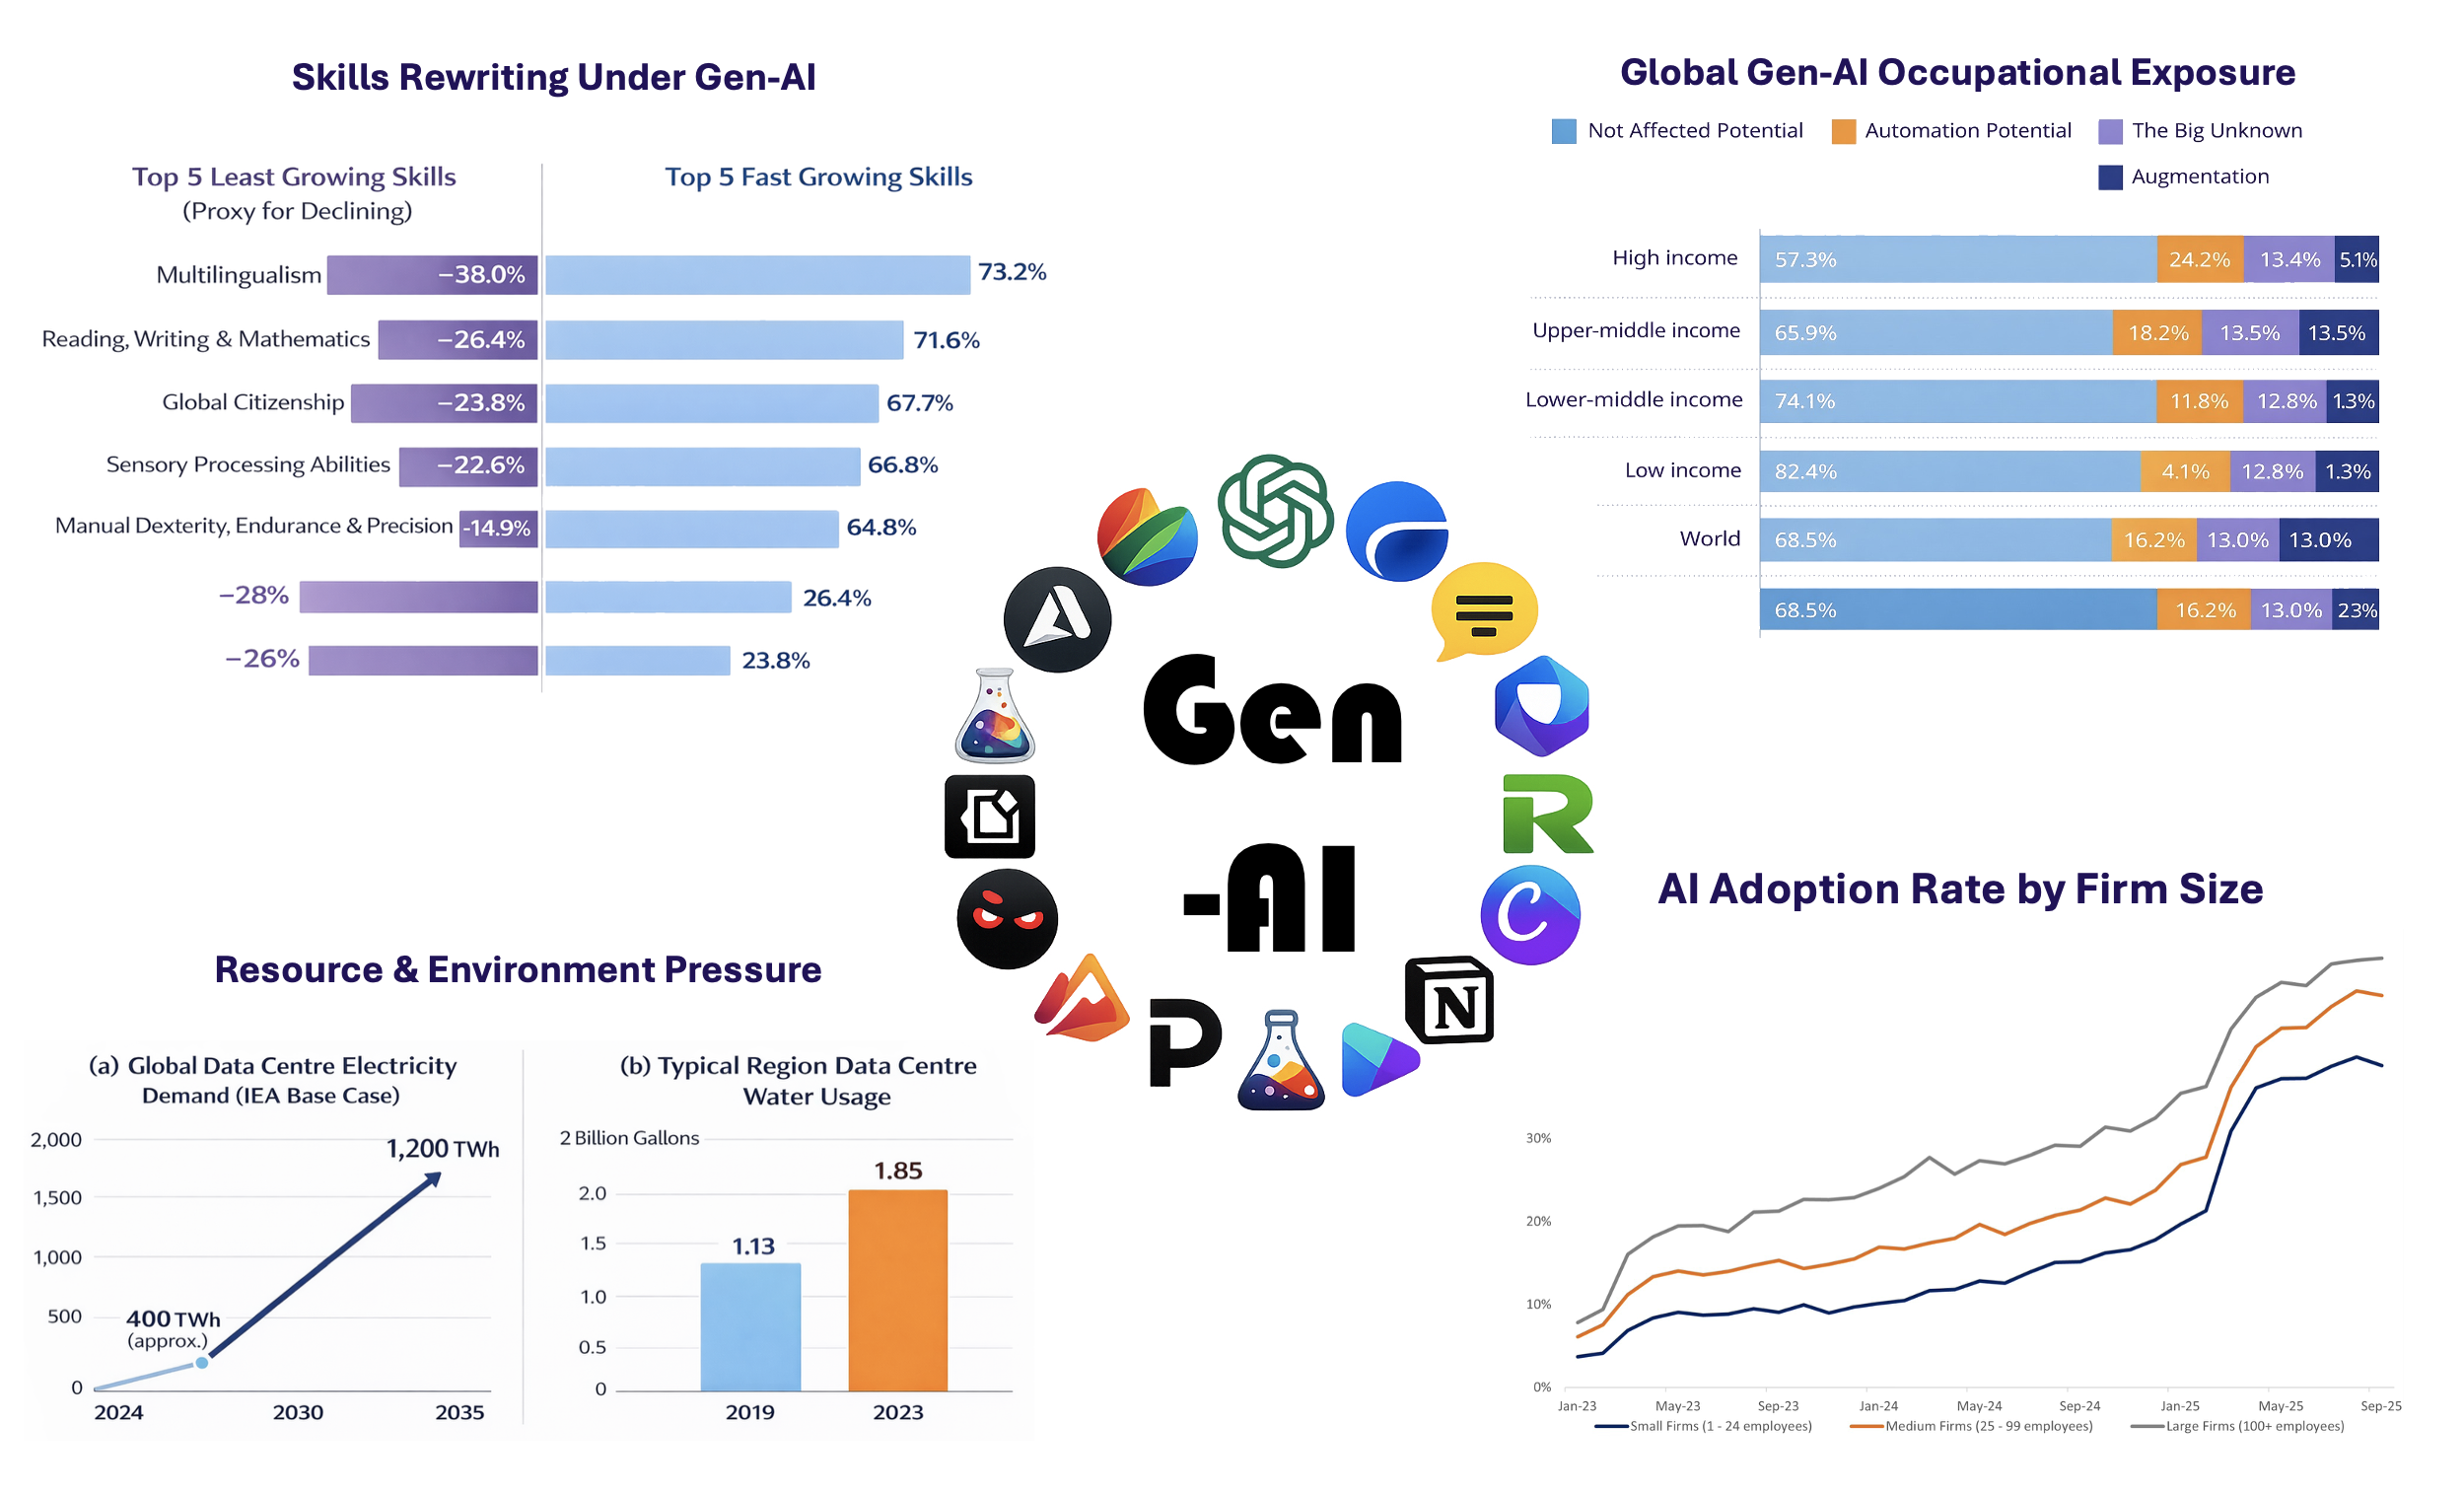
\includegraphics[width=0.98\linewidth]{gen-AI_impact_evidence.png}
  \caption{Gen-AI Impact Evidence$^1$}
  \label{fig:Gen-AI Impact Evidence}
\end{figure}

\noindent 在此背景下，本研究基于数据驱动连接将劳动力市场变化与教育决策。研究首先分析不同职业的任务变化与技能需求演化，再将结果转化为对学校与具体培养项目可操作的调整方案，涵盖课程内容、实践训练、考核设计、师资配置以及使用规范、署名与致谢等风险管理内容。通过多指标评估与不确定性分析，研究旨在提供更稳健的建议，并构建可复用的决策框架，以适用于多类型培养项目。

\subsection{我们的工作}

\begin{center}
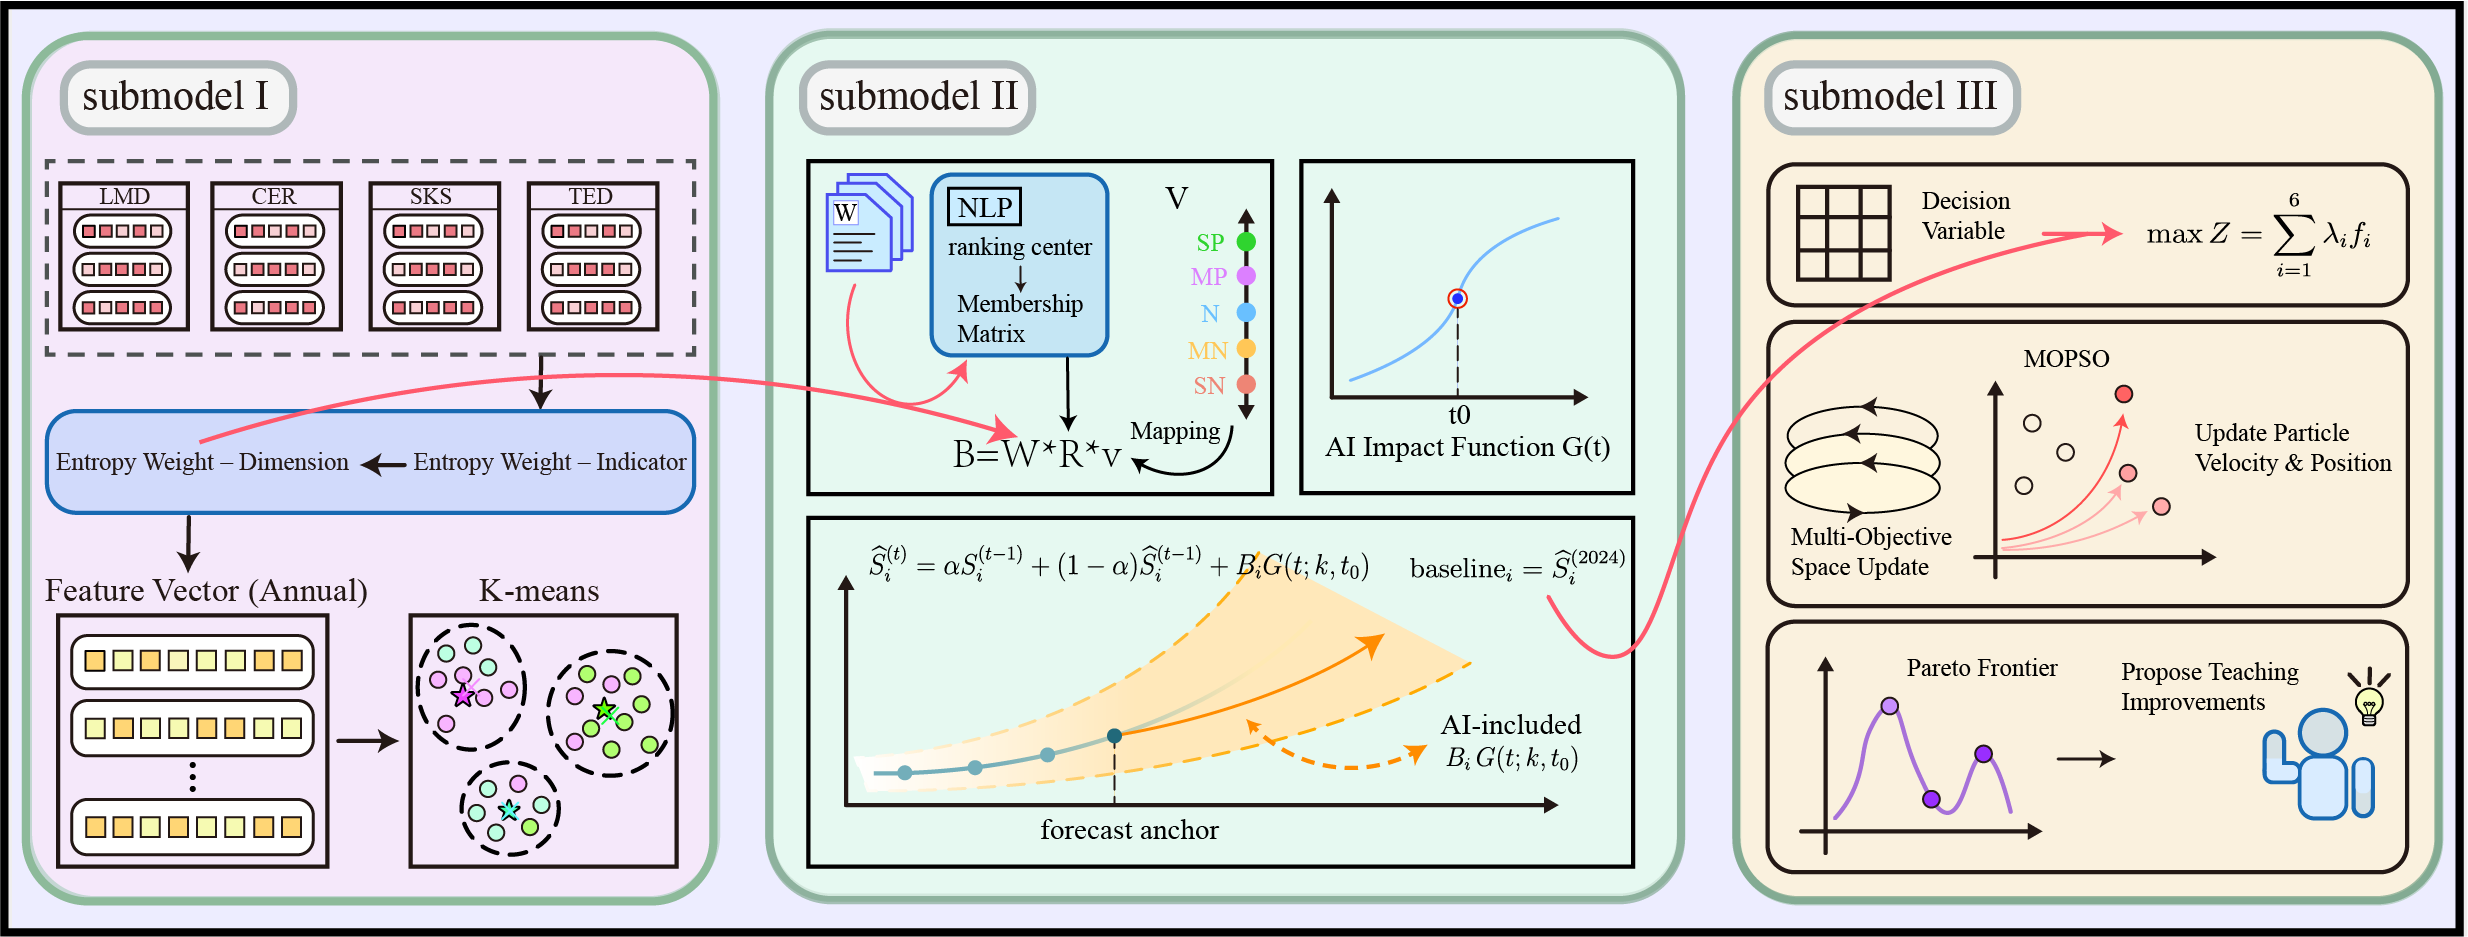
\includegraphics[width=\linewidth]{fig_framework.png}
\captionof{figure}{按工作所属职业类别标签（STEM，Trade or Arts）着色的职业二维 t-SNE 可视化结果。图中虚线圈表示聚类结果。}
\label{fig_framework.png}
\end{center}




%%----------------------------------------------------------------------------------
\subsection{问题重述}
\noindent\textbf{问题1：}在大量职业中识别出最值得重点研究、且能够代表关键变化类型的职业对象，并确保最终覆盖 STEM、技工（Trade）与艺术（Arts）三大门类各一项。

\noindent\textbf{问题2：}基于可靠数据和既有研究，构建可量化模型，预测生成式AI对三类职业发展的影响方向与强度，得出可解释的预测与趋势判断。


\noindent\textbf{问题3：}分别针对大学、职业学校与艺术院校各选一个具体项目，在前面职业趋势与Gen-AI影响分析基础上，形成三套面向校方领导的可执行建议。









%%----------------------------------------------------------------------------------
%%----------------------------------------------------------------------------------
\section{假设与合理性说明}


\noindent\textbf{Assumption 1：数据准确}\\
\noindent\textbf{Justification：}本文依赖 BLS、NCES、CSD 与 O*NET 等权威公开数据。
这些数据作为职业与教育端的基础输入。
本文假定统计口径一致，且相关数据库在长期更新过程中保持指标定义与采集方法的连续性，并假定未来不会出现导致口径系统性重构的重大制度调整或统计方法变更。
残余误差主要体现为随机噪声而非系统偏差。
这样的设定不会改变跨职业与跨年份的相对比较结论。

\medskip
\noindent\textbf{Assumption 2：指标体系全面，并忽略无指标的影响}\\
\noindent\textbf{Justification：}本文采用多维度指标体系。
该体系覆盖劳动力需求、经济回报、技能结构与技术依赖等核心维度。
指标体系用于刻画职业差异与演化特征。
本文假定未纳入的变量影响较小。
这些变量对最终综合评价与优化结论的边际贡献有限。
不会导致决策方向发生系统性反转。



\medskip
\noindent\textbf{Assumption 3：生成式AI影响随普及逐步增强并最终趋稳。}\\
\noindent\textbf{Justification：}新技术的发展通常分为三个阶段。
分别是试用、扩散与成熟阶段。本文据此假定生成式AI的影响规律。它对职业任务与技能需求的影响强度随采用率提高而增强。到成熟阶段后 影响强度会逐渐稳定。这样的设定让未来情景分析能够体现时间节奏。
避免将影响过程视为一次性突变。

\medskip
\noindent\textbf{Assumption 4：院校改革可由少量连续比例变量近似刻画。}\\
\noindent\textbf{Justification：}为保证模型具有可操作性，本文用课程模块占比与招生变化等连续变量描述培养方案。本文假定在预算与结构约束内，这些变量对就业能力、学习质量、普惠与资源利用、伦理合规等目标的作用方向稳定。同时作用机制具有可解释性。因此多目标权衡结果可作为政策与管理层面的配置参考。


%%----------------------------------------------------------------------------------
%%----------------------------------------------------------------------------------
\section{数据来源与预处理}

\subsection{数据来源}
\noindent 为保证结论具有可追溯性与可复现性，如表\ref{tab:data_sources_cn}所示，本文统一使用四个权威公开数据库作为数据基础，分别覆盖劳动力市场结果、高等教育供给与学生产出，以及职业层面的任务与技能画像，从而支撑后续的聚类、综合评价与情景分析。

\noindent\textbf{BLS（劳动力市场与薪酬）。} 
美国劳工统计局（Bureau of Labor Statistics, BLS）提供职业层面的就业与工资统计（如 OEWS 体系），可用于度量职业的就业规模、薪酬水平与随时间变化的趋势特征，是本文劳动力需求与收入回报类指标的核心来源。

\noindent\textbf{NCES（教育机构与学籍统计）。} 美国国家教育统计中心（National Center for Education Statistics, NCES）通过 IPEDS 等体系提供高校与职业院校的机构层面信息与年度统计数据，用于刻画院校属性，并作为连接教育端数据的标准化键值与背景信息来源。

\noindent\textbf{College Scorecard Database, CSD（教育产出与收益）。} 美国教育部 College Scorecard 数据库提供院校层面及部分专业层面的完成率、债务与还款、毕业后收入等指标，用于衡量不同教育路径的经济回报与负担水平，并服务于“从教育到职业”的路径评估。

\noindent\textbf{O*NET（职业任务与技能）。} O*NET OnLine 提供职业层面的任务描述、技能与能力要求、技术技能等结构化信息。本文使用该库构建职业任务与技能特征，并为刻画职业对生成式人工智能的潜在暴露程度提供可操作的代理变量。

\begin{table}[htbp]
\centering
\caption{数据来源与其在建模流程中的作用概览}
\label{tab:data_sources_cn}
\renewcommand{\arraystretch}{1.15}
\setlength{\tabcolsep}{6pt}
\begin{tabularx}{\linewidth}{@{}l X X@{}}
\toprule
\textbf{数据源} & \textbf{提供内容} & \textbf{本文用途} \\
\midrule
BLS & 职业层面就业与工资统计 & 构建劳动力需求与薪酬回报类指标 \\
NCES & 院校属性、学籍与产出统计 & 院校特征刻画与教育端数据标准化连接 \\
CSD & 完成率、债务、毕业收入等 & 教育路径回报与负担能力评估 \\
O*NET OnLine & 职业任务、能力与技术技能 & 职业任务-技能图像与 Gen-AI 暴露代理指标 \\
\bottomrule
\end{tabularx}
\end{table}

\subsection{数据预处理}
\noindent 
为保证不同数据来源与年份之间的可比性，本文对原始职业数据样本进行两步清洗与缺失值处理。第一步，剔除就业人数少于 $50{,}000$ 的职业以避免小样本造成的评估结果不稳定。第二步，对缺失数据采用分层处理策略：首先在职业层面设定缺失率阈值进行样本筛选，若某职业关键指标缺失率超过10\%,则认为其信息不足以支撑可靠评估并予以剔除；对于缺失率未超过阈值的职业，采用同一类别、同一年份下该指标的均值填补缺失值。该方法在控制噪声的同时尽量保留样本规模，为后续聚类分析与综合评价提供了一致且可复现的数据基础。

% （可选一句实现备注：如涉及跨年货币变量，可统一换算为不变价以增强可比性；建议放脚注或附录以节省篇幅。）









%%----------------------------------------------------------------------------------
%%----------------------------------------------------------------------------------
\section{符号说明}
\begin{table}[H]
\centering
\caption{符号说明}
\label{tab:notations_ultra_core_all_short}
\renewcommand{\arraystretch}{1.06}
\setlength{\tabcolsep}{6pt}
\begin{tabular}{p{0.22\linewidth} p{0.66\linewidth} p{0.08\linewidth}}
\hline
\noalign{\vskip 2mm}
\textbf{符号} & \textbf{含义说明} & \textbf{单位} \\
\noalign{\vskip 2mm}
\hline

$\mathrm{score}_i^{(t)}$ & 在年份$t$，职业$i$的综合得分 & -- \\
$\bar{\mathbf{w}}$ & 六维指标体系的平均维度权重向量 & -- \\
$K$ & 聚类数与职业类型数 & count \\

$\mathbf{R}_j$ & 职业或类型 $j$ 的隶属度矩阵 & -- \\
$\mathbf{v}$ & 影响等级分值向量 & -- \\
$B_j^{(t)}$ & 年份 $t$ 职业或类型 $j$ 的 AI 影响系数 & -- \\
$G(t;k,t_0)$ & 宏观 AI 冲击强度函数 采用 Logistic 形式 & -- \\
$k,t_0$ & Logistic 参数 加速率与拐点年份 & year \\

$\mathbf{x}$ & 院校层决策向量 课程结构与招生调整 & -- \\
$f_1,\dots,f_6$ & 六项目标函数 & -- \\
$\lambda_i$ & 目标权重系数 & -- \\
$Z$ & 综合目标函数 & -- \\
$l_i,h_i$ & 决策变量上下界 & -- \\
$\alpha,p,\beta$ & 关键参数 约束耦合与非线性敏感与折减系数 & -- \\
$C_i$ & 单位成本系数 & -- \\
$P_1,P_2$ & 约束罚项 & -- \\

\hline
\noalign{\vskip 1.5mm}
\end{tabular}
\end{table}



%%----------------------------------------------------------------------------------
%%----------------------------------------------------------------------------------
\section{多目标优化模型}
\subsection{Submodel I：基于熵权法与K-means的与代表性职业识别}

\subsubsection{指标选择}
\noindent 子模型 I 首先构建统一的指标体系，用于刻画在Gen-AI持续发展背景下，不同职业在过去 $n$ 年内的演化特征。令 $i = 1, \dots, m$ 表示职业索引，$t \in {t_1, \dots, t_n}$ 表示年份索引。对于每一个职业对应年份的观测，如表\ref{tab:dim_notations_all}所示，研究汇总劳动力市场需求、经济回报、技能结构以及技术依赖四个维度的原始指标值。



\newcommand{\DimHeader}[1]{%
  \noalign{\vskip 2pt}
  \cdashline{1-3}
  \noalign{\vskip 6pt}
  \multicolumn{3}{c}{\textbf{\textit{#1}}} \\
  \noalign{\vskip 6pt}
  \cdashline{1-3}
  \noalign{\vskip 2pt}
}

\captionsetup[table]{skip=12pt}



\begin{table}[H]
\centering
\caption{Indicator System of Submodel I}
\label{tab:dim_notations_all}
\renewcommand{\arraystretch}{1.08} % 原 1.15：略微收紧行距
\setlength{\tabcolsep}{30pt}       % 列间距保持不变
\begin{tabularx}{\linewidth}{@{}l X c@{}}
\toprule
\noalign{\vskip 1.2mm} % 原 2mm
\textbf{Symbol} & \textbf{Indicator Definition} & \textbf{Unit} \\
\noalign{\vskip 1.2mm} % 原 2mm
\midrule
\noalign{\vskip 0.6mm} % 原 1mm

\DimHeader{Dim1: Labor Market Demand (LMD)}
$\mathrm{LMD1}_{i}^{(t)}$ & Employment population size & — \\
$\mathrm{LMD2}_{i}^{(t)}$ & Employment growth rate & \% \\
$\mathrm{LMD3}_{i}^{(t)}$ & Unemployment rate & \% \\
\noalign{\vskip 0.8mm} % 原 1.2mm

\DimHeader{Dim2: Compensation and Economic Return (CER)}
$\mathrm{CER1}_{i}^{(t)}$ & Median annual salary & USD/year \\
$\mathrm{CER2}_{i}^{(t)}$ & Salary growth rate & \% \\
$\mathrm{CER3}_{i}^{(t)}$ & Income dispersion ratio & \% \\
$\mathrm{CER4}_{i}^{(t)}$ & Education-return ratio & \% \\
$\mathrm{CER5}_{i}^{(t)}$ & Middle-to-high income premium & \% \\
\noalign{\vskip 0.8mm} % 原 1.2mm

\DimHeader{Dim3: Skill Structure (SKS)}
$\mathrm{SKS1}_{i}^{(t)}$ & Share of high-skill positions & \% \\
$\mathrm{SKS2}_{i}^{(t)}$ & Skill update frequency & 1/year \\
\noalign{\vskip 0.8mm} % 原 1.2mm

\DimHeader{Dim4: Technology Dependence (TED)}
$\mathrm{TED1}_{i}^{(t)}$ & Digital tool adoption rate & \% \\
$\mathrm{TED2}_{i}^{(t)}$ & Automation potential index & - \\
$\mathrm{TED3}_{i}^{(t)}$ & Technology investment intensity & USD/year \\
$\mathrm{TED4}_{i}^{(t)}$ & Workflow standardization level & index \\
\noalign{\vskip 1.0mm} % 原 1.5mm
\bottomrule
\end{tabularx}
\end{table}


\noindent 
由于2025年的数据存在较多缺失，我们从数据源中收集到200多个岗位从2015年至2024年的数据评估最近10年的行业发展情况，并为每个职业标注类别标签。为统一单位，将负面指标$\mathrm{LMD3}_{i}^{(t)}$和$\mathrm{CER3}_{i}^{(t)}$转化后，我们使用$min-max$方法将数据归一化。在此基础上，利用归一化后的数据实现两个核心目标：其一，将多维指标整合为单一年份的综合得分，从而确保不同职业及不同时期之间的结果具备可比性；其二，结合职业的当前发展水平与聚类特征，从各类别中筛选出具有代表性的典型职业。

\noindent 为规避主观赋权带来的偏差，本文采用熵权法（EWM）确定指标权重并计算各职业的综合得分。EWM会给“职业—年份”面板数据中离散度更高的指标分配更高权重，以提供更强的区分信息辨别职业差异。假设第$j$个指标的熵权由面板数据计算得出，记为$w_j$，则职业$i$在年份t的年度综合得分可定义为

\begin{equation}
\mathrm{score}_i^{(t)}=\sum_{j=1}^{d} w_j\, x_{ij}^{(t)} .
\label{eq:score}
\end{equation}

\noindent 把每个职业各年度的综合得分依次衔接，可以得到该职业的多年度综合得分轨迹向量

\begin{equation} 
\mathrm{score}_i = \big[\mathrm{score}_i^{(t_1)},\mathrm{score}_i^{(t_2)}, \dots, \mathrm{score}_i^{(t_n)}\big]. 
\end{equation}

\begin{center}

\includegraphics[width=0.7\linewidth]{MCM:ICM/Elbow_Method.png}
\captionof{figure}{肘部法确定聚类数图}
\label{fig:Elbow_Method}
\end{center}

\noindent 为了识别出具有代表性的职业类型，我们依据职业近期得分轨迹的相似程度开展聚类分析。具体操作时，使用${score}_i$作为每个职业$i$的特征向量，对所有职业的特征向量集合$\{score_i\}$进行K-means聚类，把所有职业划分为K个组别，得到STEM、trade、arts三类工作的不同分布特征。最终综合考虑工作所属类别在聚类组中的占比与该工作与聚类中心的距离，从每个组别选取最具代表性的工作职业。如图\ref{fig:Elbow_Method}所示，聚类的组别数量由肘部法确定为3。

% 移除figure浮动环境，改用center环境固定位置，保留所有原有格式

\begin{center}

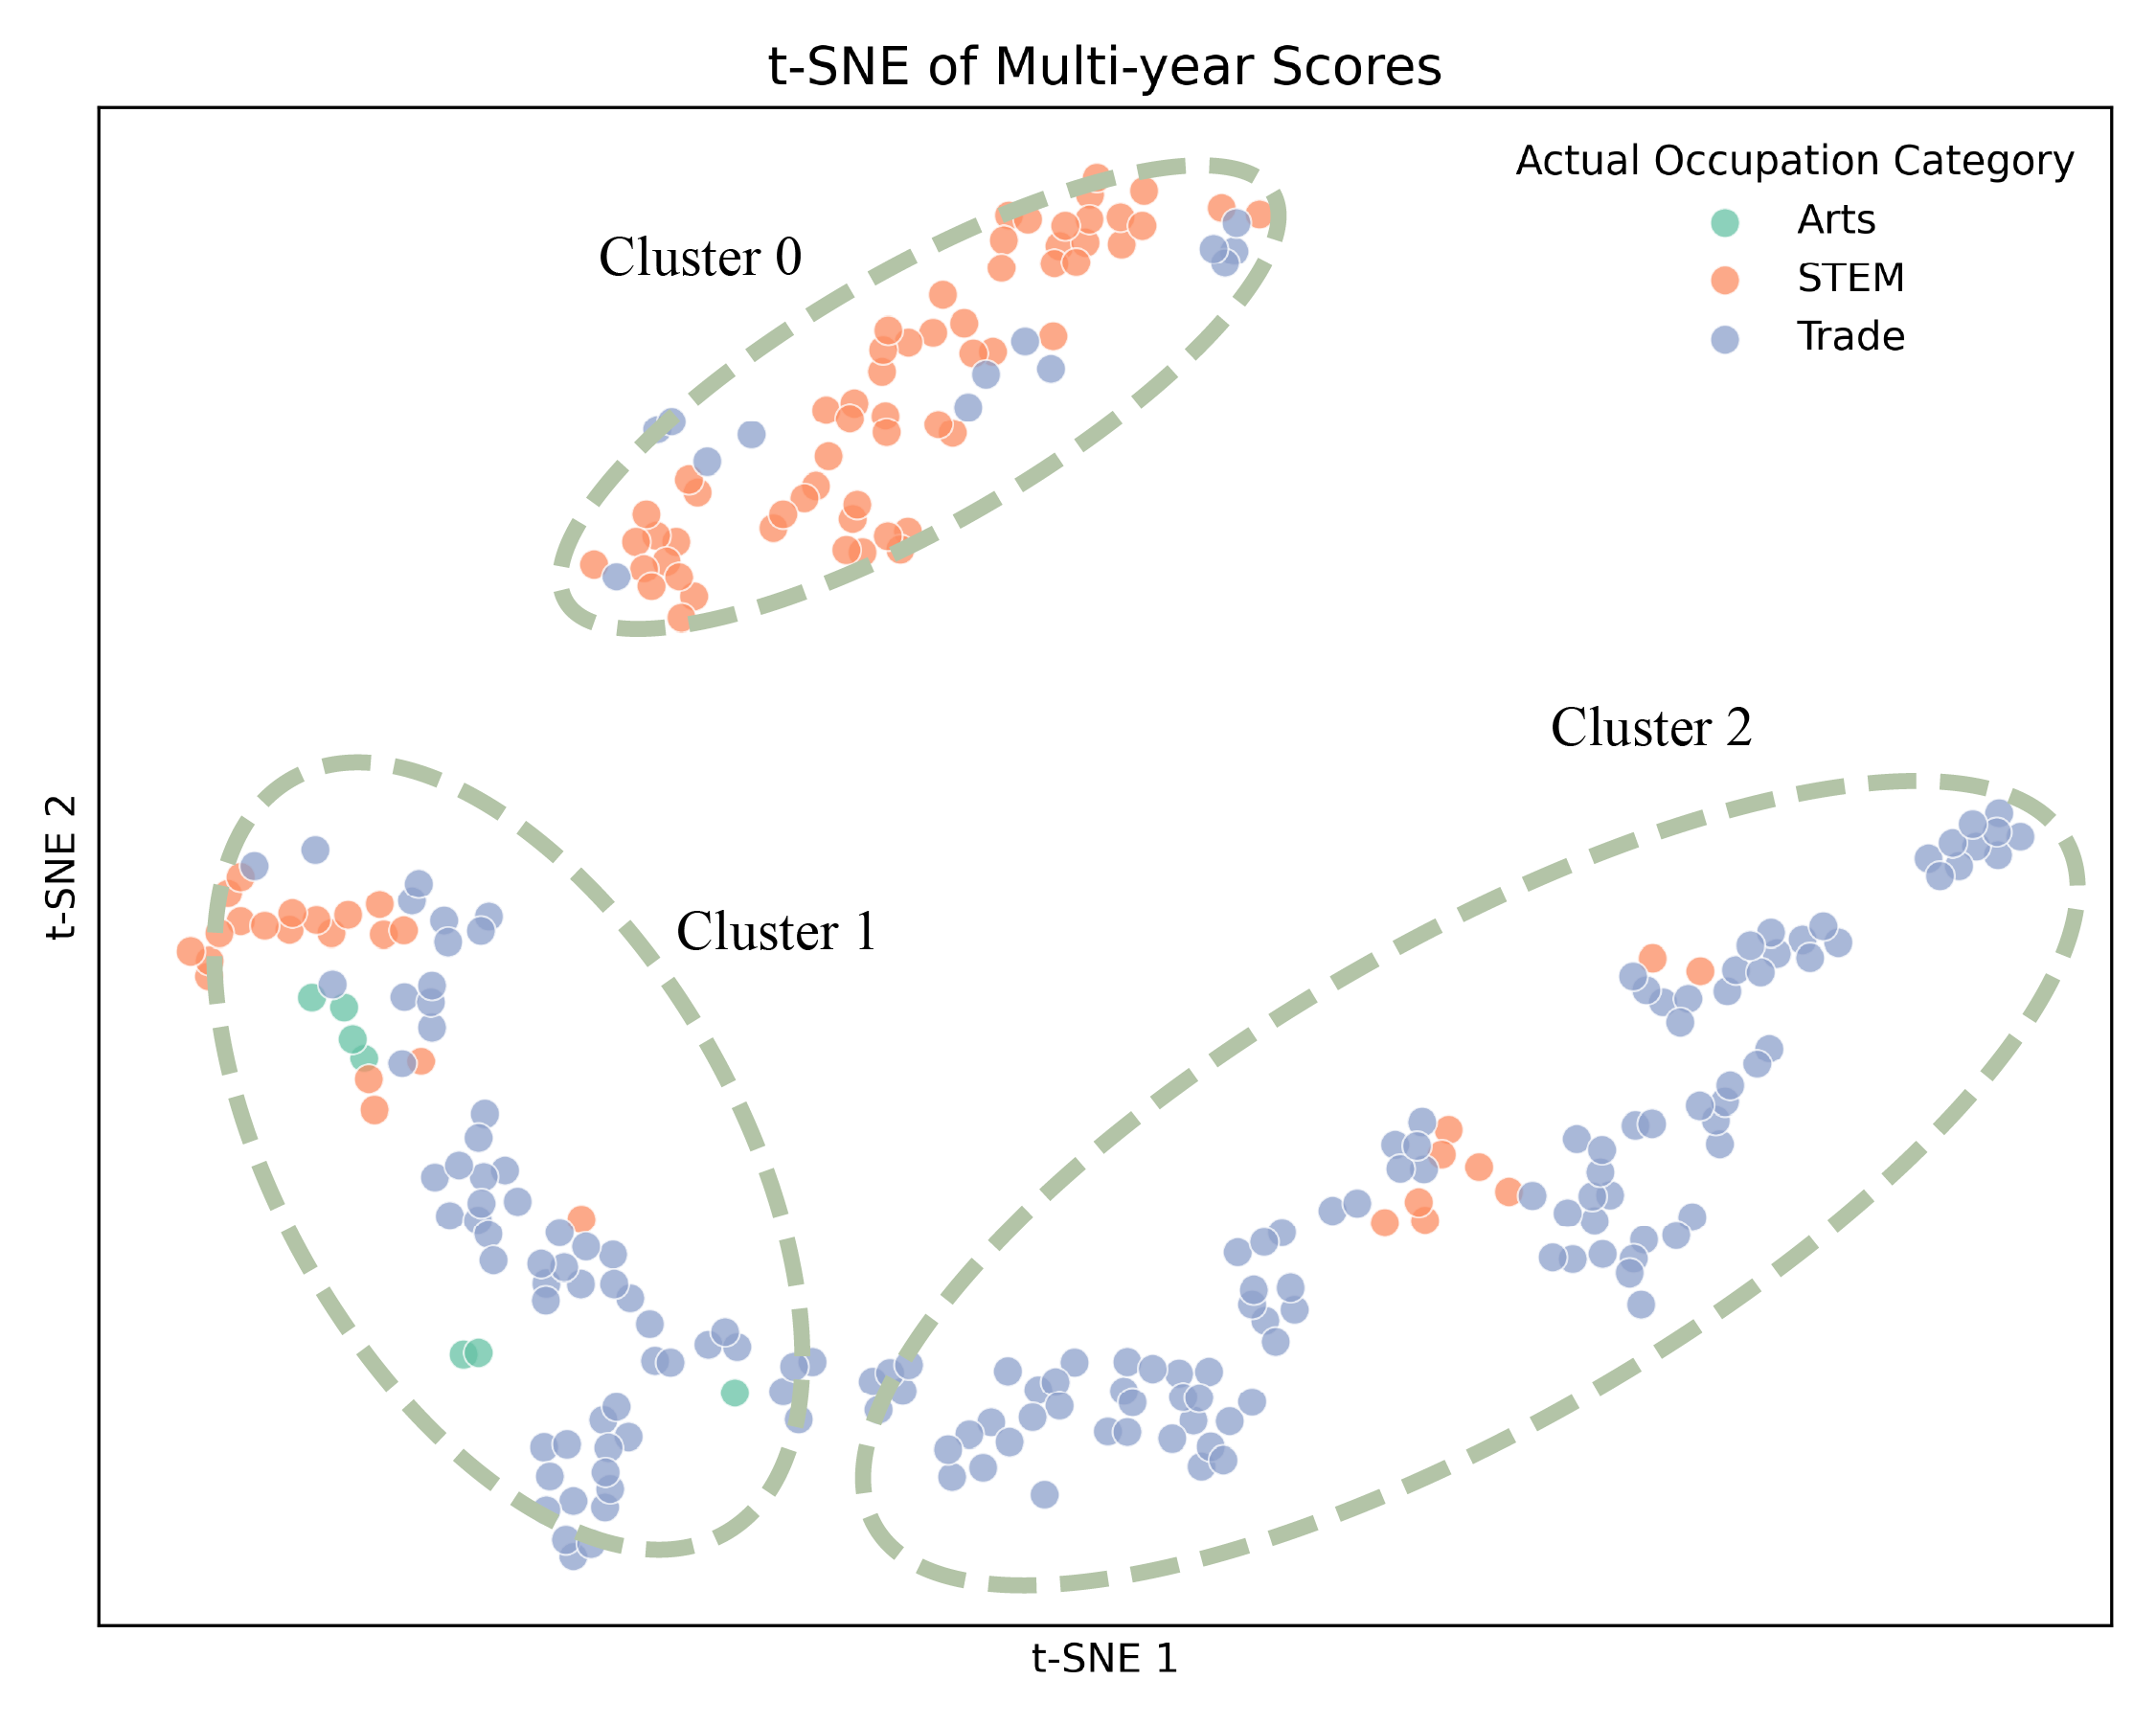
\includegraphics[width=0.7\linewidth]{fig_tsne_Kmeans.png}

\captionof{figure}{按工作所属职业类别标签（STEM，Trade or Arts）着色的职业二维 t-SNE 可视化结果。图中虚线圈表示聚类结果。}

\label{fig:tsne_clusters}

\end{center}


\subsubsection{结果：类型解释、代表性职业与趋势预测}
\noindent 为直观呈现高维综合指标空间的聚类结构，本文采用t-SNE算法将职业样本映射至二维平面可视化，结果如图\ref{fig:tsne_clusters}所示。图中三簇数据点呈现出清晰的分离边界，说明在综合指标构成的特征空间中，不同职业类型具有相对稳定的聚类结构，而非沿单一维度连续分布。基于聚类结果，本文选取各聚类簇中与聚类中心最近，且所属职业类别在聚类组别中数量占比较大的工作作为每类别的代表。最终第一簇以铁路维护工（trade类）为代表，第二簇以管理分析师（STEM类）为代表，第三簇以平面设计师（arts类）为代表。

\begin{center}

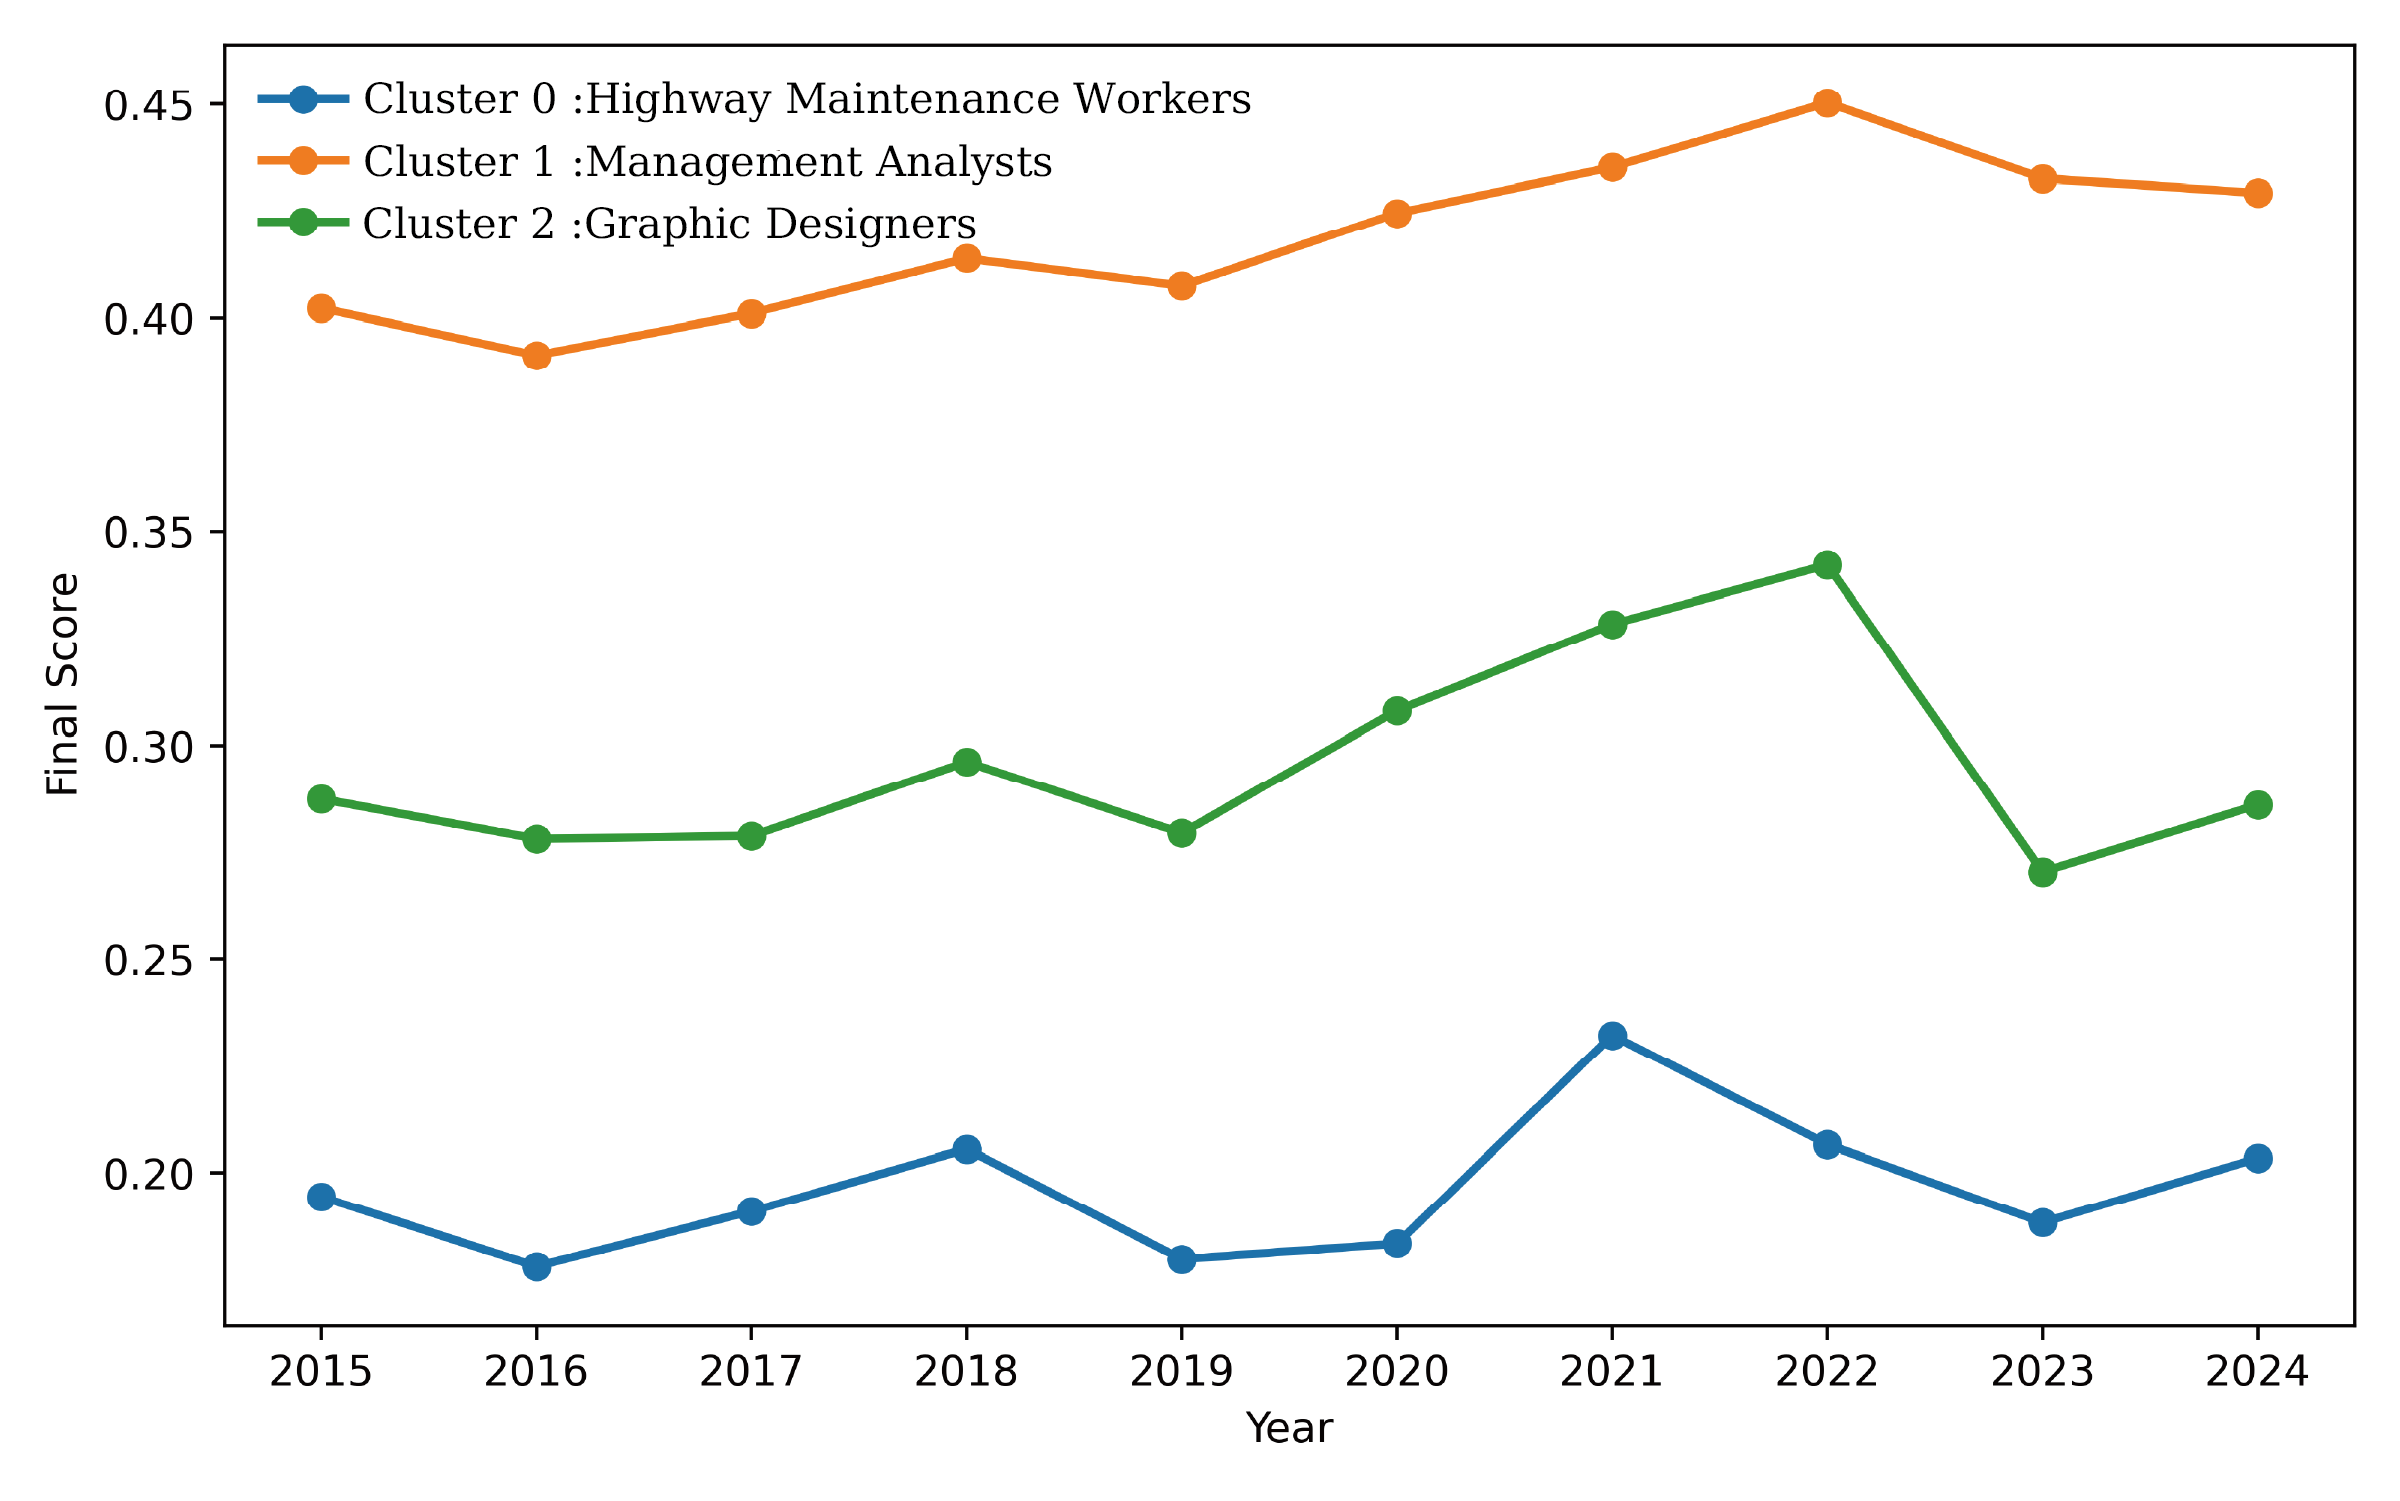
\includegraphics[width=0.7\linewidth]{fig_year_scores.png}

\captionof{figure}{三类代表性职业的年度综合评分变化趋势图。}

\label{fig:tsne_clusters}

\end{center}

\noindent 如图所示，我们选取的三个职业的综合得分呈现出稳定且层次分明的长期趋势，同时伴随年度正常波动。其中管理分析师多年保持较高综合得分，需求信号更强、教育回报更优；铁路维护工综合得分偏低，自动化暴露度高且技能更新慢；平面设计师得分居中，但未来受AI冲击最大，高端与低端的需求分化最严重。

\begin{table}[H]  % 将 [htbp] 改为 [H]，强制固定位置
\centering
\caption{职业类型：解释摘要、类规模与代表性职业。}
\label{tab:cluster_profile}
\begin{tabular}{p{0.12\linewidth} p{0.52\linewidth} p{0.12\linewidth} p{0.18\linewidth}}
\hline
Cluster & Interpretation & Size & Representative occupation \\
\hline
C0 (Trade) &
就业规模大但增长缓慢；教育回报中等；技术依赖处于低到中等水平且技能更新较慢。以标准化、经验导向为主的工作在生成式AI背景下面临更高的替代风险。 &
47--4051 &
铁路维护工 \\
\hline
C1 (STEM) &
岗位增长快、薪酬高、教育回报强；数字工具使用频繁、技术投资强度高且高技能岗位占比高。较强的人力资本与“技术互补”使其综合得分保持高位，岗位被替代风险较低。 &
13--1111 &
管理分析师 \\
\hline
C2 (Arts) &
收入波动大且薪酬差距显著；教育回报呈现分化；技术依赖不均衡且自动化风险较低；整体得分处于中等水平，但不确定性更高并存在更明显的尾部风险。 &
27--1024 &
平面设计师 \\
\hline
\end{tabular}
\end{table}

\noindent 最终，我们通过子模型I分析不同类别的工作的特征，从trade, STEM和arts三个职业类别中分别选择铁路维护工、管理分析师和平面设计师作为代表，并在后续模型中分析Gen-AI对它们未来的影响以及高等教育机构调整培养方案的方向。

%%----------------------------------------------------------------------------------
\subsection{Submodel II:}
\subsubsection{Gen-AI影响的模糊综合评价}

Gen-AI会对不同的职业的影响具有显著差异性。部分职业将随人工智能的发展实现快速增长，部分职业受其影响相对有限，还有部分职业面临被人工智能部分替代的趋势。上述职业发展特征的变化，将对高等教育机构相关专业的人才培养方案形成直接影响。为明确各职业的未来发展趋势，并为高等教育机构制定受人工智能影响行业的人才培养改革策略提供依据，本文基于Submodel I 多维度的基础数据，采用Fuzzy Comprehensive Evaluation(FCE)方法，对AI在不同维度下对各职业的影响效应展开量化评估。我们根据Submodel I得到评价集
\begin{equation} 
U=\{\mathrm{Dim1},\mathrm{Dim2},\mathrm{Dim3},\mathrm{Dim4}\}.
\end{equation}

同样，我们沿用Submodel I中的每年权重，得到历年权重集
\begin{equation} 
W^{(t)}=\big[w_1^{(t)}, w_2^{(t)}, w_3^{(t)}, w_4^{(t)}] .
\end{equation}

我们设定了5个可能的评价结果
\begin{equation} 
\begin{aligned}
V=\{\,&\text{Strong Positive Impact, Moderate Positive Impact, Neutral Impact,} \\
&\text{Moderate Negative Impact, Strong Negative Impact}\},
\end{aligned}
\end{equation}
并给它们赋予分数$\{0.2, 0.1, 0, -0.1, -0.2\}$，以便我们量化综合影响。同时规定每个等级中心点为$\{0.08,0.04,0,-0.04,-0.08\}$。

为减少隶属度矩阵$R$完全依赖人工设定的主观性，我们利用关于未来工作变化的研究[！插入文献！Ai L B Y, Ai W B. GPTs are GPTs: An Early Look at the Labor Market Impact Potential of Large Language Models By admin No Comments[J]. 2023. and so on（笔记p9）]，使用Natural Language Processing (NLP)技术提取文献关键词，并与我们为每个维度设定的关键词对照，衡量职业$i$的$j$维度受到的影响
\begin{equation} 
y_{ij}=\frac{\mathrm{positive\_word}-\mathrm{negative\_word}}{\mathrm{total\_word}}.
\end{equation}
该比值的分子是正面关键词与负面关键词的差值，用于衡量Gen-AI对未来的是正面影响还是负面影响。分母用于消除语料长度差异。最终我们利用$y_{ij}$映射反映AI对各维度影响的隶属矩阵。

通过对现有研究的分析和评价结果设计，我们使用三角隶属函数
\begin{equation}
r_{jd}^{(i)}=\max\!\left(1-\frac{|y_{ij}-c_d|}{d_0},\,0\right)
\end{equation}
将文本数据映射到隶属矩阵 $\mathbf{R}_{i}\in[0,1]^{4\times 5}$ 上。其中$r_{jd}^{(i)}$表示AI对职业$i$的$j$维度的影响最终在等级$d$上的概率，$c_d$为其等级中心，$d_0$为半宽度，在本情景中取值为0.4。

当 $y_{ij}$ 越接近等级中心 $C_d$， 其对等级 $d$ 的隶属度越高，并随距离线性衰减。当偏离超过半宽度 $d_0$ 时隶属度截断为0，从而抑制远距离等级的非物理贡献。在此基础上，我们结合Submodel I的类别评分结果与职业现实约束对 $\mathbf{r}_{jd}^{(i)}$ 做小幅人工校准，用来纠正文本证据可能存在的偏置。同时确保冲击方向与职业画像保持一致性与可解释性。

\noindent
根据NLP、隶属函数和人工微调后的结果，我们给出Trade、STEM与Arts三类职业板块的隶属矩阵，用于后续量化综合影响：

\begin{align}
\mathbf{R}_{\text{trade}} &=
\begin{bmatrix}
0.05 & 0.15 & 0.60 & 0.15 & 0.05\\
0.05 & 0.10 & 0.65 & 0.15 & 0.05\\
0.10 & 0.15 & 0.60 & 0.10 & 0.05\\
0.05 & 0.10 & 0.70 & 0.10 & 0.05
\end{bmatrix}, \label{eq:R_trade}\\
\mathbf{R}_{\text{STEM}} &=
\begin{bmatrix}
0.35 & 0.40 & 0.15 & 0.07 & 0.03\\
0.30 & 0.45 & 0.15 & 0.07 & 0.03\\
0.40 & 0.40 & 0.12 & 0.06 & 0.02\\
0.55 & 0.30 & 0.10 & 0.04 & 0.01
\end{bmatrix}, \label{eq:R_stem}\\
\mathbf{R}_{\text{arts}} &=
\begin{bmatrix}
0.08 & 0.22 & 0.20 & 0.30 & 0.20\\
0.06 & 0.20 & 0.25 & 0.29 & 0.20\\
0.20 & 0.25 & 0.30 & 0.20 & 0.05\\
0.30 & 0.40 & 0.22 & 0.06 & 0.02
\end{bmatrix}. \label{eq:R_arts}
\end{align}

\subsubsection{AI 冲击函数拟合与参数标定}

AI对职业的影响还和AI发展技术速度和普及程度有关。考虑到生成式人工智能的扩散通常呈现缓慢起步 — 快速加速 — 最终饱和的阶段性特征，我们采用 Logistic 扩散函数刻画宏观AI冲击强度的时间演化，并将其作为 Submodel II 的统一时间驱动：
\begin{equation}
G(t;k,t_0)=\frac{1}{1+\exp\!\left[-k\left(t-t_0\right)\right]}.
\label{eq:logistic_shock}
\end{equation}
其中，$t$ 为日历年份，$k$ 表示扩散加速速率，$t_0$ 为拐点年份，满足 $G(t_0;k,t_0)=0.5$，对应冲击从低强度向高强度过渡的中心时刻。依据相关研究$^{[这里也要引用]}$我们拟合出AI冲击函数的参数$k=0.8, t_0=2027$.

\subsubsection{时间序列模型预测职业未来发展}

Submodel I中，我们观察发现不同职业的当前发展轨迹各不相同，却保持相对稳定。我们在这里深入分析各职业的发展规律，并结合AI的影响共同预测职业的未来发展情况。由于我们只有过去10年的数据，因此Submodel II 中采用平滑时间序列分析提取过去10年的$score_i$基线趋势。由于直到2024年，AI冲击函数的影响始终小于0.1，我们可以认为基线数据没有受到AI的影响。时间序列的预测步骤如下所示：

\noindent \textbf{(1) 基线序列单指数平滑与参数选择.}
依据 Submodel I，记 $S_i^{(t)}$ 为职业 $i$ 在年份 $t$ 的综合评分。单指数平滑的递推形式为
\begin{equation}
\widehat{S}_i^{(t)}
=\alpha S_i^{(t-1)}+(1-\alpha)\widehat{S}_i^{(t-1)},
\qquad 0<\alpha<1.
\label{eq:ses_S_cn}
\end{equation}
其中$\widehat{S}_i^{(t)}$代表职业$i$在$t$时期的单指数平滑估计值，$S_i^{(t)}$为职业$i$在$t$时期的实际观测值，$\widehat{S}_i^{(t-1)}$是职业$i$在$t-1$时期的单指数平滑估计值；$\alpha$为指数平滑系数，取值范围为$0<\alpha<1$，用于调控当期实际观测值与前期平滑估计值在当期平滑结果中的权重分配。平滑系数$\alpha$的大小直接决定权重分配：$\alpha$越大，当期实际观测值的权重越高，平滑结果对近期数据变化的反应越灵敏；$\alpha$越小，前期平滑估计值的权重越高，平滑结果的整体稳定性则越强。
为避免平滑系数的主观设定，本文设置候选集合$\alpha\in\{0.1,0.2,0.3,0.4,0.5\}$,并采用回测误差进行选择：用 $t\in[2015,2019]$ 作为训练段得到 $\widehat{S}_i^{(2019)}$，将其作为验证段的基线锚点
\begin{equation}
\mathrm{baseline}_{i}=\widehat{S}_i^{(2019)},
\end{equation}
在 $t\in[2020,2024]$ 上计算平均绝对误差
\begin{equation}
\mathrm{MAE}(\alpha)=\frac{1}{5}\sum_{t=2020}^{2024}\left|S_i^{(t)}-\mathrm{baseline}_{i}\right|,
\label{eq:mae_alpha}
\end{equation}
选择使 $\mathrm{MAE}(\alpha)$ 最小的 $\alpha$ 作为最优平滑系数。

在得到最优 $\alpha$ 后，本文使用全历史区间 $t\in[2015,2024]$ 重新平滑以形成预测基线，并将
\begin{equation}
\mathrm{baseline}_{i}=\widehat{S}_i^{(2024)}
\end{equation}
作为未来预测的无 AI 冲击基准。

\noindent \textbf{(2) 权重稳定化与职业冲击幅度的长期化.}
为减少权重年际波动对长期预测的影响，本文采用过去十年的平均权重
\begin{equation}
\bar{\mathbf{w_i}}=\frac{1}{10}\sum_{t=2015}^{2024}\mathbf{w_i}^{(t)}.
\label{eq:wbar}
\end{equation}
得到平均权重集$\overline{W}=[w_1,w_2,w_3,w_4]$
据此，将职业 $i$ 的 AI 影响幅度定义为长期结构性系数
\begin{equation}
B_i={\overline{W}}\mathbf{R}_i\mathbf{V},
\label{eq:B_longrun}
\end{equation}
其中$B_i$表示AI最终对该职业未来的整体影响。该定义使冲击幅度不随年份短期抖动，而时间变化主要通过宏观扩散驱动项 $G(t;k,t_0)$ 体现。

\noindent \textbf{(3) AI 调整预测.}
结合上一小节的 Logistic 宏观冲击强度函数 $G(t;k,t_0)$，职业 $i$ 在未来年份 $t$ 的 AI 调整后预测值定义为
\begin{equation}
S_{i,\mathrm{future}}^{(\tau)}
=\underbrace{\mathrm{baseline}_{i}}_{\text{无AI基线}}
+\underbrace{B_i\,G(t;k,t_0)}_{\text{AI 调整项}},
\label{eq:ai_adjusted_forecast_cn}
\end{equation}
其中当 AI 处于早期扩散阶段时 $G(t;k,t_0)$ 较小，预测值接近无 AI 基线；当 AI 接近成熟扩散阶段时 $G(t;k,t_0)\to 1$，预测偏移量主要由 $B_i$ 的符号与大小决定。由此，模型能够在同一框架下刻画不同职业的净增强与净替代路径，并输出可用于情景分析与敏感性分析的标准化结果。

\noindent \textbf{(4) 初始化设置.}
为保证递推可计算，平滑序列初始化取
${S}_j^{(2015)}=S_j^{(2015)}.$该初始化在年度样本有限的情形下稳健，且不额外引入难以解释的自由参数。



%%----------------------------------------------------------------------------------
\subsection{子模型 III：}
\noindent
在院校层面，为应对生成式人工智能对岗位任务结构和技能需求的重塑，本文从三类教育路径中各选取一个代表性专业作为研究对象，分别对应技工技能型、数据分析型和创意设计型人才的培养方向，具体包括职业院校A的铁道工程技术专业，综合大学B的商业分析专业，以及艺术院校C的视觉传达设计专业。

\noindent
围绕三个培养项目，我们构建了一套面向方案选择和资源配置的多目标决策框架，共包含六项优化目标。其一为核心目标，即在给定约束下最大化毕业生就业能力，以此体现该专业对劳动力市场匹配度和职业可持续性的综合贡献。其二为优化专业招生规模，实现供需适配并控制容量风险。其三为平衡利用GENAI的学习效率和学习收获，强调在有限的学习时间和成本投入下提升学习产出质量。其四为提高知识普惠程度和院校资源利用率，兼顾教育机会公平和资源配置效率。其五为控制伦理风险并保障内容原创度，将学术诚信、数据合规和生成式内容的可追溯性纳入约束和惩罚机制。其六为减少社会资源浪费，从更高层面降低使用GenAI带来的能源等外部性损失。上述目标共同构成后续多目标优化建模和政策情景比较的评价基准。

\subsubsection{多目标规划}
\noindent\textbf{目标一：最大化毕业生就业能力。}
为衡量项目与劳动力市场的综合适配程度，我们依据子模型I劳动力市场需求、经济回报、技能结构以及技术依赖的四个维度，分别选取可量化培养要素，构建就业能力指标。这些指标分别是校企合作课程比例 $x_1$、核心课程比例 $x_2$、技能认证培训课程比例 $x_3$、实践课程比例 $x_4$，并使用Dim1至Dim4的权重。目标一的表达式如下
\begin{equation}
f_1=\sum_{i=1}^{4} w_i x_i 
\end{equation}

\noindent\textbf{目标二：优化专业招生规模。}
为让招生规模贴合劳动力需求，本文使用子模型I中的就业增长率指标$\mathrm{LMD2}$作为市场需求信号，同时设定指标$x_5$为该专业招生规模的变化率。直观来看，$x_5$越接近$\mathrm{LMD2}$，供需错配的风险就越低。因此，我们建立目标二的表达式
\begin{equation}
f_2=-\bigl|x_5-\mathrm{LMD2}\bigr|
\end{equation}

\noindent\textbf{目标三：平衡学习效率与学习收获。}
为模拟数字工具对学习过程的双刃效应，本文采用模型I中的数字工具使用率指标 $\mathrm{TED1}$作为合理工具依赖水平的参照。设 $x_6$ 表示项目的 Gen-AI 使用强度，可以使用AIGC介入率或作业中AI使用频率衡量。若 $x_6$ 过高，可能带来表层化学习与能力虚高，过低则可能降低学习效率与工具素养。因此，本文以偏离惩罚形式刻画适度使用原则
\begin{equation}
f_3=-\bigl(x_6-\mathrm{TED1}\bigr)^2
\end{equation}

\noindent\textbf{目标四：提高知识普惠程度与院校资源利用率。}
对于因 Gen-AI 冲击而不得不缩减招生规模的项目，可以通过增加公共通识课程来补偿资源利用的不足。此类课程面向大众，既能够普及知识，又可通过适度收费创造收入。本文以公共通识课程比例 $x_7$ 作为指标，并以正向效用形式刻画该目标：
\begin{equation}
f_4= x_7\bigl[\max(-x_5,0)\bigr]^p
\end{equation}
对于缩招幅度较大的院校，模型会提升 $x_7$ 数值，以此减少教学资源的浪费。对于扩招阶段的专业，我们要求其专注于对自身教学与就业能力的提升。因此在假设预算充足的情况下，扩招阶段的专业的本目标为0。幂指数$p$决定缩招幅度对开设通识课目标的影响。

\noindent\textbf{目标五：控制伦理风险并保障内容原创度。}
直观来看，AI使用强度的增大会提高抄袭、署名不清与伦理风险。我们设$x_8$为 AI 伦理与原创内容规范培训课程比例，希望通过规范训练，降低上述风险，同时提升原创意识。为同时体现培训投入的正效应与高强度使用AI带来的负效应，本文将目标五定义为
\begin{equation}
f_5=x_8(1-x_6)
\end{equation}

\noindent\textbf{目标六：减少社会资源浪费。}
使用AI会造成能源和水资源的额外消耗。我们用 $x_6$ 的线性项刻画资源节约效应，引入折减系数 $\beta$ 表示该效应的相对权重，目标六表达式为
\begin{equation}
f_6=-\beta x_6
\end{equation}
尽管我们希望学生使用AI时考虑环境因素，但这不应该成为制约AI使用的主要因素。因此$\beta$ 取0.3。较小值既体现 AI 的效率增益，也避免过度抑制教育创新。\\

\noindent\textbf{综合目标函数}
为统一权衡六项目标，本文采用加权和法构造总体效用函数
\begin{equation}
\max Z=\sum_{i=1}^{6}\lambda_i f_i
\end{equation}
其中主目标f1的权重$\lambda_1$设为0.5，其余权重设为0.1。
约束条件定义为
\begin{equation}
\text{s.t.}
\begin{cases}
l_i\le x_i\le h_i,\qquad i=1,2,\dots,8 \\
x_1+x_2+x_3+x_4+x_7+x_8\le 1\\
C_1x_1+C_2x_2+C_3x_3+C_4x_4+C_7x_7+C_8x_8\le C_0
\end{cases}
\end{equation}
\noindent 其中，第1式为各变量的边界约束；第2式为保证课程结构可行的比例约束；第3式为预算可行域约束，限制各类课程的预算不超过总预算。在边界约束方面，对于变量$x_1\sim x_6$，我们根据通常情况规定它们的常数上下限。由于项目扩招会挤压公共通识课程的资源，因此对于$x_7$，我们规定它的上限与课程扩招规模有关。对于$x_8$，由于AI风险与AI使用强度有关，因此教育机构应该保证AI伦理课程的最小教育投入，我们将它的下限与AI使用强度关联。基于以上描述，我们设计出三所教育机构的三个项目的变量上下限：

\medskip
\noindent\textbf{(1) Trade school $A$ Railroad Engineering Technology：}
\[
\mathbf{l}^{(A)}=
(0.05,\ 0.2,\ 0.05,\ 0.05,\ -0.25,\ 0,\ 0,\ \alpha x_6)
\]
\[
\mathbf{h}^{(A)}=
(0.5,\ 1,\ 0.5,\ 0.5,\ 0.25,\ 1,\ 0.5-x_7[\max(0,x_5)]^{p},\ 0.3)
\]

\medskip
\noindent\textbf{(2) University $B$ Business Analytics：}
\[
\mathbf{l}^{(B)}=
(0,\ 0.5,\ 0,\ 0,\ -0.25,\ 0,\ 0,\ \alpha x_6)
\]
\[
\mathbf{h}^{(B)}=
(0.3,\ 1,\ 0.3,\ 0.3,\ 0.25,\ 1,\ 0.5-x_7[\max(0,x_5)]^{p},\ 0.15)
\]

\medskip
\noindent\textbf{(3) Arts school $C$ Graphic Design：}
\[
\mathbf{l}^{(C)}=
(0.05,\ 0.3,\ 0.05,\ 0.05,\ -0.25,\ 0,\ 0,\ \alpha x_6)
\]
\[
\mathbf{h}^{(C)}=
(0.3,\ 1,\ 0.5,\ 0.5,\ 0.25,\ 1,\ 1-x_7[\max(0,x_5)]^{p},\ 0.3)
\]
其中$\alpha$为调控AI强度对AI伦理课程影响的系数，设置为0.3，$p$为衡量扩招对公共通识课程影响的系数，设置为1.5。

\noindent 对于约束条件3，$C_i$为课程$x_i$的对应成本，$C_0$为项目全年的总预算。项目的总预算与招生规模和职业现状有关。我们规定
\[
\mathbf{C}=
(15,\ 5,\ 10,\ 10,\ -2,\ 1)
\]
将模型II中的baseline归一化后，计算由招生规模和行业现状调控后的总预算
\[
\mathbf{C_0}=
20(1+x_5)baseline
\]

\subsubsection{PSO for Solving the Curriculum Allocation Problem}
\noindent 为在连续空间中求解上述优化模型，本文采用粒子群算法搜索最优课程配比。其中每个粒子表示一个可行方案
$\mathbf{X}=(x_1,\dots,x_8)$，
并以综合目标值 $Z$ 作为适应度函数：
\[
\mathrm{fitness}(\mathbf{X})=Z
\]

\noindent 我们根据约束条件构造惩罚项。针对课程配比约束，定义惩罚项
\[
P_1=\eta\sqrt{\max\!\left(x_1+x_2+x_3+x_4+x_7+x_8-1,\ 0\right)}
\]
其中$\eta=10$。针对预算约束，定义惩罚项
\[
P_2=\max\!\left(C_1x_1+C_2x_2+C_3x_3+C_4x_4+C_7x_7+C_8x_8-C_0,\ 0\right)
\]
于是 PSO 实际优化的目标为
\[
\max \ \mathrm{fitness}(\mathbf{X})-P_1-P_2.
\]
通过查询所选的三所教育机构的特征，我们设定它们的初始解：
\[
\mathbf{X}^{(A)}=
(0.16,\ 0.32,\ 0.14,\ 0.17,\ 0.06,\ 0.30,\ 0.10,\ 0.11)
\]
\[
\mathbf{X}^{(B)}=
(0.10,\ 0.55,\ 0.05,\ 0.05,\ 0.13,\ 0.70,\ 0.15,\ 0.10)
\]
\[
\mathbf{X}^{(C)}=
(0.10,\ 0.35,\ 0.08,\ 0.22,\ -0.08,\ 0.50,\ 0.15,\ 0.10)
\]
\noindent 我们设置粒子数$N$=100，最大迭代次数$K$=200，个体学习因子$c_1$=2，群体学习因子$c_2$=2，第$k$步的惯性权重$\omega^{(k)}=\omega_{\max}-\dfrac{\omega_{\max}-\omega_{\min}}{K}\,k$。其中$\omega_{\max}$=0.9, $\omega_{\min}$=0.4，表示惯性权重随步数递增线性衰退，粒子群由前期的探索模式转换为后期的保守模式。
算法在达到最大迭代次数 $K$ 时停止，并输出最优解 $\mathbf{X}^\ast$。通过最优解得到新的效用值 $\mathbf{Z}^\ast$。我们通过相对提升率量化方案改进效果：
\[
\mathrm{Improvement}=\frac{Z^\ast-Z}{Z},
\]
并基于提升效果和对各目标得分变化的分析，为教育机构提出调整建议。
（画雷达图）



\section{灵敏度分析}
\noindent 本节检验Model III在高校偏好权重$\boldsymbol{\lambda}$变化时的稳健性。基准设定以就业为核心目标，与之相比，不同类型高校的使命与约束存在系统性差异，最优政策解$\mathbf{x}^\star$可能会对$\boldsymbol{\lambda}$产生敏感反应。为将这一问题从情景描述转化为可重复的敏感性实验，本文采用离散画像与局部微扰相结合的两层设计。首先构建三类使命画像作为代表性权重点，再在每个画像附近对权重进行$\pm10\%$的扰动，观察最优解与目标达成情况的变化幅度，这种做法和范例中通过小幅调整权重验证模型鲁棒性的思路一致。

\subsection{目标}

\noindent 设归一化目标向量为

\[\mathbf{F}(\mathbf{x})=\big(f_1(\mathbf{x}),f_2(\mathbf{x}),f_3(\mathbf{x}),f_4(\mathbf{x}),f_5(\mathbf{x}),f_6(\mathbf{x})\big)^\top,\]

\noindent 综合效用为

\begin{equation}Z(\mathbf{x};\boldsymbol{\lambda})=\sum_{k=1}^{6}\lambda_k f_k(\mathbf{x}),\qquad\lambda_k\ge 0,\ \sum_{k=1}^{6}\lambda_k=1,\label{eq:lambda_utility}\end{equation}

\noindent 其中$\mathbf{x}$是政策变量，$f_k(\cdot)$对应Q3中的六项目标。本文构建三类高校画像并设定对应权重，具体如下：

\[
\begin{aligned}
\boldsymbol{\lambda}^{(A)}&=(0.25,\,0.10,\,0.30,\,0.05,\,0.15,\,0.15)
&&\text{对应科研型高校，侧重前沿创新与资源节约},\\
\boldsymbol{\lambda}^{(B)}&=(0.15,\,0.10,\,0.10,\,0.15,\,0.25,\,0.25)
&&\text{对应伦理与环保型高校，侧重限制AI使用、强化治理与可持续发展},\\
\boldsymbol{\lambda}^{(C)}&=(0.15,\,0.20,\,0.05,\,0.30,\,0.15,\,0.15)
&&\text{对应商业化型高校，侧重市场敏感、创收导向并兼顾合规要求}.
\end{aligned}
\]

\noindent 分别求解得到最优政策解$\mathbf{x}^{\star(A)}$、$\mathbf{x}^{\star(B)}$、$\mathbf{x}^{\star(C)}$，进而得到对应的目标达成向量$\mathbf{F}(\mathbf{x}^{\star(\cdot)})$，用于从宏观层面对比使命差异引发的政策结构变化。

\noindent\subsection{局部权重微扰与量化指标}

\noindent 为避免敏感性分析沦为单纯的情景对比，本文在每个画像附近开展局部扰动。对于任意一类高校画像$\boldsymbol{\lambda}^{(p)}$，$p$取值为A、B、C，对其每一维权重进行$\pm10\%$的微调，微调后再做归一化处理，生成扰动集合$\mathcal{N}(\boldsymbol{\lambda}^{(p)})$，随后重复求解过程得到$\mathbf{x}^\star(\boldsymbol{\lambda})$。之后通过两类指标量化敏感性：

\noindent\textbf{（1）目标达成敏感度：} 针对每个目标$k$定义相对变化率

\begin{equation}
\Delta_k(\boldsymbol{\lambda})=\frac{f_k(\mathbf{x}^\star(\boldsymbol{\lambda}))-f_k(\mathbf{x}^\star(\boldsymbol{\lambda}^{(p)}))}{\left|f_k(\mathbf{x}^\star(\boldsymbol{\lambda}^{(p)}))\right|+\varepsilon}
\end{equation}

\noindent 并采用$\max_{\boldsymbol{\lambda}\in\mathcal{N}(\boldsymbol{\lambda}^{(p)})}|\Delta_k(\boldsymbol{\lambda})|$表示最坏情况下的波动幅度。

\noindent\textbf{（2）政策结构敏感度：} 通过解的归一化距离描述政策组合的变化

\begin{equation} 
 D(\boldsymbol{\lambda})=\frac{\|\mathbf{x}^\star(\boldsymbol{\lambda})-\mathbf{x}^\star(\boldsymbol{\lambda}^{(p)})\|_2}{\|\mathbf{x}^\star(\boldsymbol{\lambda}^{(p)})\|_2+\varepsilon}
\end{equation}

\noindent 若在$\pm10\%$的扰动下，$D(\boldsymbol{\lambda})$与各$\Delta_k$的数值均维持在较小水平，说明结论对偏好权重具备鲁棒性；若数值出现明显增大，表明政策建议对偏好设定较为敏感，此时应按照画像分层的方式输出政策包，优先选用在邻域内保持近似最优的稳健解。范例中也提到，参数组合或扰动可能放大系统响应，需要关注这类交互影响。



%%----------------------------------------------------------------------------------
%%----------------------------------------------------------------------------------
\section{优势和不足}
\subsection{优势}
\noindent\textbf{优势一 可追溯性与可执行性}

模型构建了职业识别、影响量化、方案优化的闭环流程。首先从数据中筛选出代表性职业，再明确生成式人工智能对各职业影响的方向与强度，最后在预算和结构约束下，输出课程设置与招生安排的可落地方案，确保结论可复核、建议能落地。

\medskip

\noindent\textbf{优势二 可解释性与低复杂度}

模型整合了综合评分、聚类分型、模糊评价与扩散函数等成熟方法，参数含义清晰易懂。输出结果可对应需求、回报、技能及技术依赖等多个维度，既方便评审人员理解与对比，也能将同一流程复用到其他职业或项目中。

\medskip

\noindent\textbf{优势三 稳健性与适配性}

通过高校使命画像结合局部权重扰动的敏感性实验，检验方案对偏好设定的稳定性。同时借助约束惩罚机制，确保解决方案符合现实边界、具备可行性，可针对不同院校类型分层输出政策包，提升模型的迁移能力与落地效果。

\subsection{不足}

\noindent\textbf{不足一 聚合偏差与异质性不足}

对每个代表性职业采用单一影响系数，可能忽略同一职业内部的岗位分工差异、单位技术采用程度差异以及任务重组差异。因此，模型更适合用于不同职业类型间的相对比较与趋势判断，难以对细分岗位进行精准预测。

\medskip

\noindent\textbf{不足二 参数依赖与情景敏感}

扩散函数的关键参数，比如拐点与加速率，会影响预测变化出现的时间范围。隶属度映射也依赖语料库与规则设定，因此结果需结合基准情景与敏感性分析共同呈现，避免对单一发展路径做出绝对化解读。








%%----------------------------------------------------------------------------------
%%----------------------------------------------------------------------------------
\section{结论}
本文提出面向院校决策的闭环框架，涵盖职业趋势识别、Gen-AI影响量化及培养方案优化。以STEM、Trade与Arts三大门类各一代表职业为分析主线，基于四大公开数据库（BLS、NCES/IPEDS、College Scorecard、O*NET），分三种子模型实施。
子模型I构建多维指标体系，通过熵权法计算职业年度综合得分，结合得分轨迹开展K-means聚类，识别稳定职业类型并确定代表职业。
子模型II采用模糊综合评价生成隶属度矩阵与标准化AI影响系数，结合Logistic扩散函数与指数平滑基线，实现未来职业发展的可解释预测。
子模型III搭建院校多目标优化模型，以课程与招生调整为决策变量，在预算及可行性约束下，通过粒子群算法求解最优培养方案。
整体流程将职业变化转化为院校可落地政策包，通过偏好权重扰动检验优化建议在不同办学使命下的稳健性与可迁移性。



\begin{appendices}
\section{附录一}




%%----------------------------------------------------------------------------------
%%-------------------------------------------------------------------------
\end{appendices}




%%----------------------------------------------------------------------------------
%%----------------------------------------------------------------------------------
\section{参考文献}
\noindent [1]  World Economic Forum, The Future of Jobs Report 2023; International Labour Organization, Generative AI and Jobs: A Refined Global Index of Occupational Exposure; International Energy Agency, Energy and AI; IT Brew; U.S. Census Bureau BTOS-based firm AI-use time series, documented in CES Working Paper 24-16 and summarized in SBA Office of Advocacy.

\noindent [2] Frey \& Osborne, automation risk by occupation; McKinsey, AI task automation share; WEF, Future of Jobs Report; OECD, AI exposure index; NBER, GenAI task-exposure studies; OpenAI, task exposure classification (2023)

\noindent [3] Forecasting the Impacts of AI R\&D Acceleration: Results of a Pilot Study



%%----------------------------------------------------------------------------------
%%----------------------------------------------------------------------------------
\AImatter

\begin{ReportAiUse}{9}
\bibitem{AI1}
\noindent \textbf{使用工具：} OpenAI ChatGPT（模型：GPT-5.2 Thinking）\\
\textbf{使用目的：} 用于概念解释、语言支持以及代码排错建议。该工具未用于生成或伪造任何数据，也未用于替代团队对模型方案、参数设定、计算与结论解释的独立判断。所有最终内容均由团队复核确认。

\vspace{4pt}
\begin{enumerate}
  \item \textbf{OpenAI ChatGPT}\\
  \textbf{Query1：}\texttt{<Please explain to me in simple terms the meaning of Pareto optimization and the scenarios of its use>}\\
  \textbf{Output：} 对“帕累托优化”进行了通俗解释，强调其多目标权衡含义，即在不使至少一个目标变差的前提下无法继续改进其他目标，并概述其常见应用场景，如资源配置、谈判决策与公共政策权衡等。

  \item \textbf{OpenAI ChatGPT}\\
  \textbf{Query1：}\texttt{<I will send you the paragraphs of the paper written in Chinese and ask you to translate the content of the paragraphs into English. Requirements: standardized use of language, no grammatical errors, no mistakes or omissions.>}\\
  \textbf{Output：} 确认可将团队提供的中文段落翻译为规范英文表达，并尽量保证语法正确、信息不遗漏。

  \item \textbf{OpenAI ChatGPT}\\
  \textbf{Query1：}\texttt{<Next I’m going to talk about sending you a piece of Python code and ask you to check the code for syntax errors.>}\\
  \textbf{Output：} 对团队提供的 Python 代码给出排错建议，涉及潜在未定义变量、数组与标量维度不匹配风险、绘图前需检查 NaN/inf 等数值有效性，以及字体在不同环境中的可用性问题并给出替代设置建议。

  \item \textbf{OpenAI ChatGPT}\\
  \textbf{Query1：}\texttt{<Could you briefly tell me the format of the Memo?>}\\
  \textbf{Output：} 给出 Memo 的常见格式要点，包括标题栏（To/From/Date/Subject）与正文部分的简洁结构建议，强调用短段落或要点列表提升可读性。
\end{enumerate}

\vspace{4pt}
\noindent \textbf{责任与边界声明：} 团队对报告中的模型构建、参数选择、数据处理、计算结果、图表生成与结论建议承担全部责任。AI 输出仅作为辅助建议，所有引用与事实性表述均由团队核对确认后使用；AI 未被用于生成、补全或推断任何未经团队计算/验证的数值结果或数据来源。

\end{ReportAiUse}

\end{document}
